\documentclass[12pt]{article}
\usepackage[left=1cm, right=1cm, top=2cm,bottom=1.5cm]{geometry} 

\usepackage[parfill]{parskip}
\usepackage[utf8]{inputenc}
\usepackage[T2A]{fontenc}
\usepackage[russian]{babel}
\usepackage{enumitem}
\usepackage[normalem]{ulem}
\usepackage{amsfonts, amsmath, amsthm, amssymb, mathtools,xcolor}
\usepackage{blkarray}

\usepackage{tabularx}
\usepackage{hhline}

\usepackage{accents}
\usepackage{fancyhdr}
\pagestyle{fancy}
\renewcommand{\headrulewidth}{1.5pt}
\renewcommand{\footrulewidth}{1pt}

\usepackage{graphicx}
\usepackage[figurename=Рис.]{caption}
\usepackage{subcaption}
\usepackage{float}

%%Наименование папки откуда забирать изображения
\graphicspath{ {./images/} }

%%Изменение формата для ввода доказательства
\renewcommand{\proofname}{$\square$  \nopunct}
\renewcommand\qedsymbol{$\blacksquare$}

%%Изменение отступа на таблицах
\addto\captionsrussian{%
	\renewcommand{\proofname}{$\square$ \nopunct}%
}
%% Римские цифры
\newcommand{\RN}[1]{%
	\textup{\uppercase\expandafter{\romannumeral#1}}%
}

%% Для удобства записи
\newcommand{\MR}{\mathbb{R}}
\newcommand{\MC}{\mathbb{C}}
\newcommand{\MQ}{\mathbb{Q}}
\newcommand{\MN}{\mathbb{N}}
\newcommand{\MZ}{\mathbb{Z}}
\newcommand{\MTB}{\mathbb{T}}
\newcommand{\MTI}{\mathbb{I}}
\newcommand{\MI}{\mathrm{I}}
\newcommand{\MCI}{\mathcal{I}}
\newcommand{\MJ}{\mathrm{J}}
\newcommand{\MH}{\mathrm{H}}
\newcommand{\MT}{\mathrm{T}}
\newcommand{\MU}{\mathcal{U}}
\newcommand{\MV}{\mathcal{V}}
\newcommand{\MB}{\mathcal{B}}
\newcommand{\MF}{\mathcal{F}}
\newcommand{\MW}{\mathcal{W}}
\newcommand{\ML}{\mathcal{L}}
\newcommand{\MP}{\mathcal{P}}
\newcommand{\VN}{\varnothing}
\newcommand{\VE}{\varepsilon}
\newcommand{\dx}{\, dx}
\newcommand{\dy}{\, dy}
\newcommand{\dz}{\, dz}
\newcommand{\dd}{\, d}


\theoremstyle{definition}
\newtheorem{defn}{Опр:}
\newtheorem{rem}{Rm:}
\newtheorem{prop}{Утв.}
\newtheorem{exrc}{Упр.}
\newtheorem{problem}{Задача}
\newtheorem{lemma}{Лемма}
\newtheorem{theorem}{Теорема}
\newtheorem{corollary}{Следствие}

\newenvironment{cusdefn}[1]
{\renewcommand\thedefn{#1}\defn}
{\enddefn}

\DeclareRobustCommand{\divby}{%
	\mathrel{\text{\vbox{\baselineskip.65ex\lineskiplimit0pt\hbox{.}\hbox{.}\hbox{.}}}}%
}
%Короткий минус
\DeclareMathSymbol{\SMN}{\mathbin}{AMSa}{"39}
%Длинная шапка
\newcommand{\overbar}[1]{\mkern 1.5mu\overline{\mkern-1.5mu#1\mkern-1.5mu}\mkern 1.5mu}
%Функция знака
\DeclareMathOperator{\sgn}{sgn}

%Функция ранга
\DeclareMathOperator{\rk}{\text{rk}}
\DeclareMathOperator{\diam}{\text{diam}}


%Обозначение константы
\DeclareMathOperator{\const}{\text{const}}

\DeclareMathOperator{\codim}{\text{codim}}

\DeclareMathOperator*{\dsum}{\displaystyle\sum}
\newcommand{\ddsum}[2]{\displaystyle\sum\limits_{#1}^{#2}}

%Интеграл в большом формате
\DeclareMathOperator{\dint}{\displaystyle\int}
\newcommand{\ddint}[2]{\displaystyle\int\limits_{#1}^{#2}}
\newcommand{\ssum}[1]{\displaystyle \sum\limits_{n=1}^{\infty}{#1}_n}

\newcommand{\smallerrel}[1]{\mathrel{\mathpalette\smallerrelaux{#1}}}
\newcommand{\smallerrelaux}[2]{\raisebox{.1ex}{\scalebox{.75}{$#1#2$}}}

\newcommand{\smallin}{\smallerrel{\in}}
\newcommand{\smallnotin}{\smallerrel{\notin}}

\newcommand*{\medcap}{\mathbin{\scalebox{1.25}{\ensuremath{\cap}}}}%
\newcommand*{\medcup}{\mathbin{\scalebox{1.25}{\ensuremath{\cup}}}}%

\makeatletter
\newcommand{\vast}{\bBigg@{3.5}}
\newcommand{\Vast}{\bBigg@{5}}
\makeatother

%Промежуточное значение для sup\inf, поскольку они имеют разную высоту
\newcommand{\newsup}{\mathop{\smash{\mathrm{sup}}}}
\newcommand{\newinf}{\mathop{\mathrm{inf}\vphantom{\mathrm{sup}}}}

%Скалярное произведение
\newcommand{\inner}[2]{\left\langle #1, #2 \right\rangle }
\newcommand{\linsp}[1]{\left\langle #1 \right\rangle }
\newcommand{\linmer}[2]{\left\langle #1 \vert #2\right\rangle }

%Подпись символов снизу
\newcommand{\ubar}[1]{\underaccent{\bar}{#1}}

%% Шапка для букв сверху
\newcommand{\wte}[1]{\widetilde{#1}}
\newcommand{\wht}[1]{\widehat{#1}}

%%Трансформация Фурье
\newcommand{\fourt}[1]{\mathcal{F}\left(#1\right)}
\newcommand{\ifourt}[1]{\mathcal{F}^{-1}\left(#1\right)}

%%Символ вектора
\newcommand{\vecm}[1]{\overrightarrow{#1\,}}

%%Пространстов матриц
\newcommand{\mat}[2]{\operatorname{Mat}_{#1\times #2}}


%%Взятие в скобки, модули и норму
\newcommand{\parfit}[1]{\left( #1 \right)}
\newcommand{\modfit}[1]{\left| #1 \right|}
\newcommand{\sqparfit}[1]{\left\{ #1 \right\}}
\newcommand{\normfit}[1]{\left\| #1 \right\|}

%%Функция для обозначения равномерной сходимости по множеству
\newcommand{\uconv}[1]{\overset{#1}{\rightrightarrows}}
\newcommand{\uconvm}[2]{\overset{#1}{\underset{#2}{\rightrightarrows}}}


%%Функция для обозначения нижнего и верхнего интегралов
\def\upint{\mathchoice%
	{\mkern13mu\overline{\vphantom{\intop}\mkern7mu}\mkern-20mu}%
	{\mkern7mu\overline{\vphantom{\intop}\mkern7mu}\mkern-14mu}%
	{\mkern7mu\overline{\vphantom{\intop}\mkern7mu}\mkern-14mu}%
	{\mkern7mu\overline{\vphantom{\intop}\mkern7mu}\mkern-14mu}%
	\int}
\def\lowint{\mkern3mu\underline{\vphantom{\intop}\mkern7mu}\mkern-10mu\int}

%%След матрицы
\DeclareMathOperator*{\tr}{tr}

\makeatletter
\renewcommand*\env@matrix[1][*\c@MaxMatrixCols c]{%
	\hskip -\arraycolsep
	\let\@ifnextchar\new@ifnextchar
	\array{#1}}
\makeatother


%% Переопределение функции хи, чтобы выглядела более приятно
\makeatletter
\@ifdefinable\@latex@chi{\let\@latex@chi\chi}
\renewcommand*\chi{{\@latex@chi\smash[t]{\mathstrut}}} % want only bottom half of \mathstrut
\makeatletter

\begin{document}
\lhead{Математический анализ - \RN{2}}
\chead{Косухин О.Н.}
\rhead{Семинар - 5}
\section*{Метод Остроградского}

\begin{problem}(\textbf{Д1898})
	Выделить алгебраическую часть интеграла:
	$$
		\dint \dfrac{x^2 + 1}{(x^4 + x^2 + 1)^2}dx
	$$
\end{problem}

\begin{proof}
	$$
		\dint \dfrac{x^2 + 1}{(x^4 + x^2 + 1)^2}dx = \dfrac{P_2(x)}{Q_2(x)} + \dint\dfrac{P_1(x)}{Q_1(x)}dx, \, P(x) = x^2 + 1, \, Q(x) = (x^4 + x^2 + 1)^2
	$$
	У квадратного трехчлена действительных корней нет, только комплексные. Как их найти в явном виде? Домножим на $(z^2 - 1)$, тогда по формуле разности кубов:
	$$
		(z^2 - 1)(z^4 + z^2 + 1) = z^6 - 1
	$$ 
	Надо взять корни многочлена справа и выбросить корни многочлена $z^2 -1$:
	$$
		z_i = e^{2\pi i{\cdot}\frac{k}{6}}, \, k = 0,1,2,3,4,5
	$$
	Следовательно, остаются только $k =1,2,4,5$:
	$$
		e^{\frac{\pi i}{3}}, \, e^{\frac{2\pi i }{3}}, \, e^{\frac{4\pi i}{3}}, \, e^{\frac{5\pi i}{3}}
	$$
	Графически делим окружность на $6$ равных частей, выбрасываем корни для $z^2 -1$. Видно, что кратных корней нет.
	\begin{figure}[H]
		\centering
		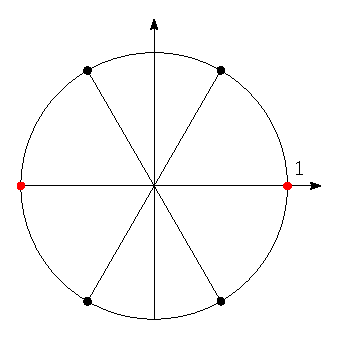
\includegraphics[width=0.25\textwidth]{MA2S5_1.eps}
		\caption{Корни многочлена $z^6 - 1$ и $z^2 - 1$.}
		\label{5_1}
	\end{figure}
	Можно было действовать по-другому. Проверим кратность корней у квадратного трехчлена:
	$$
		G(x) = x^4 + x^2 + 1 = 0, \, G'(x) = 4x^3 + 2x = 0 \Rightarrow x(4x^2 + 2) = 0 \Rightarrow x = 0, x = \pm \sqrt{-\tfrac{1}{2}} = \pm i\sqrt{\tfrac{1}{2}}
	$$
	$$
		G(0) = 1 \neq 0, \, G\left(\pm i\sqrt{\tfrac{1}{2}}\right) = \dfrac{1}{4} - \dfrac{1}{2} + 1 = \dfrac{3}{4} \neq 0
	$$
	Следовательно кратных корней нет. Тогда:
	$$
		Q	_1(x) = Q_2(x) = x^4 + x^2 + 1, \, P_2(x) = Ax^3 + Bx^2 + Cx + D, \, \deg{P_1, P_2} \leq 3
	$$
	$$
		(x^2 + 1)Q_2(x) = (3Ax^2 + 2Bx + C)Q_2^2(x) - (Ax^3 + Bx^2 + Cx + D)(4x^3 + 2x)Q_2(x) + P_1(x)Q_2^2(x) \Rightarrow
	$$
	$$
		\Rightarrow x^2 + 1 = (3Ax^2 + 2Bx + C)Q_2(x) - (Ax^3 + Bx^2 + Cx + D)(4x^3 + 2x) + P_1(x)Q_2(x)
	$$
	Нам необходимо получить уравнения на коэффициенты $A,B,C,D$, минуя $P_1(x)$. Для этого будем подставлять значения $z$ такие, чтобы $Q_2(x) = 0$:
	$$
		z \in \MC \colon z^4 + z^2 +  1 = 0 \Rightarrow z_1 = e^{\frac{\pi i}{3}},\, z_2 = e^{\frac{2\pi i }{3}}, \, z_3 = e^{\frac{4\pi i}{3}}, \, z_4 = e^{\frac{5\pi i}{3}} \Rightarrow 
	$$
	$$
		\Rightarrow Q_2(z) = 0 \Rightarrow z^2 + 1 = -(Az^3 + Bz^2 + Cz + D)(4z^3  + 2z) \Rightarrow
	$$
	 Поскольку у нас возникают слагаемые степени выше $3$, то избавимся от них:
	$$
		z^4 = -z^2 - 1 \Rightarrow z^5 = -z^3- z, \, z^6 = -z^4 - z^2 = 1
	$$
	Следовательно мы получим систему уравнений:
	$$
		z^2 + 1 = -(Az^3 + Bz^2 + Cz + D)(4z^3 + 2z) =
	$$
	$$
		 = -4A - 4B(-z^3- z) - 4C(-z^2 -1) - 4Dz^3 - 2A(-z^2 - 1) - 2Bz^3 - 2Cz^2 + 2Dz = 
	$$
	$$
		= z^3(4B - 4D - 2B) + z^2(4C +2A - 2C)+ z(4B - 2D) - 4A + 4C + 2A
	$$
	Таким образом, мы получили что два многочлена один не выше $3$-ой степени, второй не выше $3$-ей совпадают в $4$ точках $\Rightarrow$ совпадают всюду $\Rightarrow$ коэффициенты у них должны быть равны:
	$$
		\left\{
		\begin{array}{ccccc}
			z^3 \colon& 0 & = &  2B - 4D\\
			z^2 \colon& 1 & = & 2C + 2A\\
			z \colon& 0 & = & 4B - 2D\\
			1 \colon & 1 &=& 4C -2A
		\end{array}
		\right. \Rightarrow
		\left\{
		\begin{array}{ccc}
			A & = & \tfrac{1}{2} - C\\ [8pt]
			B & = & 2D  = 0\\[8pt]
			D & = & 2B  = 0\\[8pt]
			A & = & 2C - \tfrac{1}{2}
		\end{array} \Rightarrow
		\right. 		
		\left\{
		\begin{array}{ccc}
			A & = & \tfrac{1}{6} \\[8pt]
			B & = & 0 \\[8pt]
			C & = & \tfrac{1}{3} \\[8pt]
			D & = & 0
		\end{array}
		\right. 
	$$
	Следовательно, алгебраическая часть будет иметь вид:
	$$
		\dfrac{P_2(x)}{Q_2(x)} = \dfrac{1}{6}{\cdot}\dfrac{ x^3 + 2x }{x^4 + x^2 + 1}
	$$
\end{proof}
\begin{rem}
	Заметим, что функция $\dfrac{x^2 + 1}{x^4 + x^2 + 1}$ - это четная функция, тогда её производная - нечетная и наоборот, если функция четная, то её первообразная нечетная: 
	$$
		f(z) = f(-z) \Rightarrow f'(z) = -f'(-z)
	$$
	$$	
		f(z) = -f(-z) \Rightarrow \dint f(z)dz = \dint f(-z)d(-z) = F(z) = F(-z) +C
	$$
	Тогда, если раскладывать нечетную функцию на алгебраическую и трансцендентную части, то алгебраическая часть будет нечетной $\Rightarrow$ можно понять что $B$ и $D$ будут равны нулю, поскольку стоят при четных степенях. Это возможно обсудим далее.
\end{rem}

\newpage
\section*{Интегрирование некоторых иррациональных функций}
Пусть помимо операций вычитания, сложения,  умножения и деления над многочленами ещё добавили операцию извлечения корня $n$-ой степени $\Rightarrow$ мы получаем иррациональные функции. При интегрировании иррациональных функций не всегда интеграл можно посчитать, но иногда это получается. Рассмотрим сначала ситуации, когда иррациональная функция может быть сведена к рациональной.

\begin{problem}(\textbf{Д1929})
	$$
		\dint \dfrac{1 - \sqrt{x + 1}}{1 + \sqrt[3]{x + 1}}dx
	$$
\end{problem}
\begin{proof}
	Можно сообразить, что оба иррациональных выражения в отношении являются степенями корня $6$-ой степени: 
	$$
		\sqrt{x+1} = (\sqrt[6]{x + 1})^3, \, \sqrt[3]{x + 1} = (\sqrt[6]{x + 1})^2
	$$
	Сделаем замену:
	$$
		t = \sqrt[6]{x+1} \Rightarrow x = t^6 - 1, \, dx = 6t^5dt \Rightarrow
	$$
	$$
		\Rightarrow \dint \dfrac{1 - \sqrt{x + 1}}{1 + \sqrt[3]{x + 1}}dx = \dint \dfrac{1 - t^3}{1 + t^2}{\cdot}6t^5 dt = \dint \dfrac{6t^5 - 6t^8}{1 + t^2}dt = -6 \dint\dfrac{t^8 - t^5}{1 + t^2}dt
	$$
	Степень числителя выше степени знаменателя $\Rightarrow$ поделим в столбик:
	$$
		t^8 - t^5 = (t^2 + 1)(t^6 - t^4 -t^3 + t^2 + t -1) - t + 1 \Rightarrow
	$$
	$$
		\Rightarrow -6 \dint\dfrac{t^8 - t^5}{1 + t^2}dt = -6\left(\dfrac{t^7}{7} - \dfrac{t^5}{5} - \dfrac{t^4}{4} + \dfrac{t^3}{3} + \dfrac{t^2}{2} - t\right) -6\dint\dfrac{1 -t}{1 + t^2}dt
	$$
	$$
		-6\dint\dfrac{1 -t}{1 + t^2}dt = 6\dint\dfrac{t}{1 +t^2}dt - 6\dint\dfrac{1}{1+t^2}dt =  \dfrac{6}{2}\ln{(t^2 + 1)} - 6\arctg{t} + C \Rightarrow 
	$$
	$$
		\Rightarrow -6 \dint\dfrac{t^8 - t^5}{1 + t^2}dt = -6\left(\dfrac{t^7}{7} - \dfrac{t^5}{5} - \dfrac{t^4}{4} + \dfrac{t^3}{3} + \dfrac{t^2}{2} - t\right) + \dfrac{6}{2}\ln{(t^2 + 1)} - 6\arctg{t} + C, \, t = \sqrt[6]{x + 1}
	$$
\end{proof}

\begin{problem}(\textbf{Д1931})
	$$
		\dint \dfrac{\sqrt{x + 1} - \sqrt{x - 1}}{\sqrt{x + 1} + \sqrt{x - 1}}dx
	$$
\end{problem}
\begin{proof}
	В таких задачах часто помогает домножение на сопряженное слагаемое, чтобы избавиться от рациональности в знаменателе:
	$$
		\dint \dfrac{\sqrt{x + 1} - \sqrt{x - 1}}{\sqrt{x + 1} + \sqrt{x - 1}}dx = \dint\dfrac{\left(\sqrt{x + 1} - \sqrt{x - 1}\right)^2}{(x + 1) - (x - 1)}dx = \dfrac{1}{2}\dint\left(x + 1 + x- 1+ 2\sqrt{x^2 -1}\right)dx 
	$$
	Мы уже считали такой интеграл с радикалом:
	$$
		\dint \sqrt{x^2 - a^2}dx = \dfrac{x}{2}{\cdot}\sqrt{x^2 - a^2} - \dfrac{a^2}{2}\ln{\left|x + \sqrt{x^2 - a^2}\right|} + C \Rightarrow
	$$
	$$
		\Rightarrow \dfrac{1}{2}\dint\left(x + 1 + x- 1+ 2\sqrt{x^2 -1}\right)dx = \dfrac{x^2}{2} -  \dfrac{x}{2}{\cdot}\sqrt{x^2 - 1} - \dfrac{1}{2}\ln{\left|x + \sqrt{x^2 - 1}\right|} + C
	$$
\end{proof}
\begin{rem}
	Снова вспомним, что когда у нас есть простые корни, то мы можем делать замены для избавления от них:
	$$
		\sqrt{x^2 + a^2} \Rightarrow x = a\sh{t}
	$$
	$$
		\sqrt{x^2 -a^2} \Rightarrow x = a\ch{t}
	$$
	$$
		\sqrt{a^2 - x^2} \Rightarrow x = a\sin{t} \vee x = a\cos{t }
	$$
	Задачи $1937$-$1942$ могут быть сведены с помощью замен выше к интегрированию выражений от $\sin{x}$, $\cos{x}$, $\sh{x}$, $\ch{x}$. Интегрирование таких задач мы обсудим позже.
\end{rem}

\subsection*{Аналог метода Остроградского}

Рассмотрим аналог формулы Остроградского для конкретного выражения с корнями.
\begin{theorem}
	$$
		y = \sqrt{ax^2 + bx + c}, \, \dint \dfrac{P_n(x)}{y}dx = Q_{n-1}(x){\cdot}y + \lambda{\cdot}\dint\dfrac{dx}{y} 
	$$
	$$	
		\deg{P_n} = n,\, \deg{Q_{n-1}} \leq n-1, \, \lambda \in \MR 
	$$
	
\end{theorem}

\begin{problem}(\textbf{Д1946})
	$$
		\dint \dfrac{x^3 - 6x^2 +11 x - 6}{\sqrt{x^2 + 4x + 3}}dx
	$$
\end{problem}
\begin{proof}
	$$
		y = \sqrt{x^2 + 4x + 3}, \, P_3(x) = x^3 - 6x^2 + 11x - 6, \, \deg{P_3} = 3
	$$
	Тогда по формуле выше, мы получим:
	$$
		\dint \dfrac{x^3 - 6x^2 +11 x - 6}{\sqrt{x^2 + 4x + 3}}dx = (Ax^2 + Bx + C){\cdot}y + \lambda \dint \dfrac{dx}{y}
	$$
	Продифференцируем левую и правую части и посмотрим какое уравнение получится:
	$$
		\dfrac{x^3 - 6x^2 +11 x - 6}{y} = (2Ax + B){\cdot}y + (Ax^2 + Bx + C){\cdot}\dfrac{1}{2}{\cdot}\dfrac{2ax + b}{\sqrt{ax^2 +bx + c}} + \dfrac{\lambda}{y}
	$$
	Умножим обе части на $y$, тогда:
	$$
		x^3 - 6x^2 + 11x -6 = (2Ax + B){\cdot}(x^2 + 4x + 3) + (Ax^2 + Bx + C){\cdot}(x + 2) + \lambda
	$$
	Здесь можно идти несколькими путями: просто приравнять коэффициенты перед степенями, либо подставлять конкретные точки и смотреть значения в них, можно комбинированный метод использовать. Нам важно получить $A,B,C$, а существование таких коэффициентов гарантирует теорема выше.
	
	Рассмотрим коэффициент при $x^3$:
	$$
		x^3 \colon 1 = 3A \Rightarrow A = \dfrac{1}{3}
	$$
	Далее, подставим точки $x = 0, x = -1, x = -2$:
	$$
		x = -1 \Rightarrow -1 - 6 - 11 - 6 = -24 = A - B + C + \lambda
	$$ 
	$$
		x = -2 \Rightarrow -8 -24 -22 -6 = -60 = (-4A + B){\cdot}(-1)+ \lambda
	$$
	$$
		x = 0 \Rightarrow -6 = 3B + 2C + \lambda
	$$
	Теперь решим систему из полученных уравнений:
	$$
		B = 60 + \dfrac{4}{3} + \lambda \Rightarrow \dfrac{1}{3} - 60 -\dfrac{4}{3} + C = -24 \Rightarrow C = 61 - 24 = 37
	$$
	$$
		3\left(60 + \dfrac{4}{3} + \lambda\right) + 74 + \lambda = -6 \Rightarrow 4\lambda = -6 -180 -4 -74 = -264 \Rightarrow \lambda = - 66
	$$
	$$
		B = 60 + \dfrac{4}{3} - 66 = -\dfrac{14}{3}
	$$
	Таким образом, мы получаем:
	$$
		Q_2(x) = \dfrac{1}{3}x^2 -\dfrac{14}{3}x + 37 
	$$
	Посчитаем оставшийся интеграл:
	$$
		\dint \dfrac{dx}{\sqrt{x^2 +4x + 3}} = \dint \dfrac{dx}{\sqrt{(x+2)^2 -1}} = \left|x + 2 = \ch{t}, \, (x+ 2)^2 - 1 =\ch^2{t} - 1 = \sh^2{t}, \, dx = \sh{t}dt\right| =
	$$
	$$
		=\dint  1 {\cdot}dt = t + C  = \ch^{-1}(x+ 2) + C = \ln{\left|x+2 + \sqrt{x^2 + 4x + 3}\right|} + C
	$$
	$$
		\dint \dfrac{x^3 - 6x^2 +11 x - 6}{\sqrt{x^2 + 4x + 3}}dx = \left(\dfrac{1}{3}x^2 -\dfrac{14}{3}x + 37 \right){\cdot}\sqrt{x^2 + 4x + 3} - 66\ln{\left|x+2 + \sqrt{x^2 + 4x + 3}\right|} + C
	$$
\end{proof}

Есть модификация этого метода, если многочлен проступает вниз тоже. Рассмотрим следующий пример.
\begin{problem}(\textbf{Д1948})
	$$
		\dint \dfrac{dx}{x^4\sqrt{x^2 -1}}
	$$
\end{problem}
\begin{proof}
	Пусть $x > 1$, тогда сделаем замену $t = \tfrac{1}{x} \in (0,1)$, тогда:
	$$
		x = \dfrac{1}{t}, \, \sqrt{x^2 - 1} = \dfrac{\sqrt{1 - t^2}}{t}, \, dx = -\dfrac{1}{t^2}dt \Rightarrow
	$$
	$$
		\Rightarrow \dint \dfrac{dx}{x^4\sqrt{x^2 -1}} = \dint t^4{\cdot}\left(-\dfrac{1}{t^2}\right){\cdot}t{\cdot}\dfrac{1}{\sqrt{1 - t^2}}dt = -\dint \dfrac{t^3}{\sqrt{1- t^2}}dt
	$$
	Теперь можем воспользоваться теоремой:
	$$
		-\dint \dfrac{t^3}{\sqrt{1- t^2}}dt = (At^2 + Bt + C){\cdot}y + \lambda \dint\dfrac{dt}{y} 
	$$
	Продифференцируем это равенство:
	$$
		-t^3 = (2At +B){\cdot}(1 -t^2)  + (At^2 + Bt +C){\cdot}(-t) + \lambda
	$$
	$$
		\left\{
			\begin{matrix}
				t^3\colon& -1 &=& -2A &-& A  \\
				t^2\colon&  0 &=& -B &-& B  \\
				t\colon & 0 &=& 2A &-&C  \\
				1 \colon & 0 &=& B &+& \lambda  
			\end{matrix}
		\right. \Rightarrow
		\left\{
			\begin{matrix}
				A &=& \tfrac{1}{3}&&\\[5pt]
				B &=& 0&&\\[5pt]
				C &=& 2A &=& \tfrac{2}{3}\\[5pt]
				\lambda &=& -B &=& 0
			\end{matrix}
		\right.
	$$
	Таким образом, мы получим:
	$$
		-\dint \dfrac{t^3}{\sqrt{1- t^2}}dt = \left(\dfrac{1}{3}t^2 + \dfrac{2}{3}\right){\cdot}\sqrt{1-t^2} + C, \, t = \dfrac{1}{x}
	$$
\end{proof}

\begin{problem}(\textbf{Д1951})
	$$
		\dint \dfrac{a_1x^2 + b_1 x + c}{\sqrt{ax^2 + bx + c}}dx
	$$
	Когда этот интеграл представляет собой алгебраическую функцию? 
\end{problem}
\begin{proof}
	Нам необходимо понять, когда выполнено следующее:
	$$
		\dint \dfrac{a_1x^2 + b_1 x + c_1}{\sqrt{ax^2 + bx + c}}dx = (Ax + B){\cdot}y + C
	$$
	То есть, когда $\lambda = 0$ в формуле выше. Продифференцируем и умножим на корень:
	$$
		a_1 x^2 + b_1 x + c_1 = A{\cdot}y^2 + (Ax +B){\cdot}\left(ax + \tfrac{b}{2}\right)	= A(ax^2 + bx + c) + (Ax +B)\left(ax + \tfrac{b}{2}\right)
	$$
	Нужно чтобы существовали $A$ и $B$ так, чтобы выполнялось равенство выше. Найдем коэффициенты:
	$$
		\left\{
			\begin{matrix}
				x^2 \colon & a_1 &=& 2aA \\[8pt]
				x \colon & b_1 &=&  A{\cdot}b + B{\cdot}a + A{\cdot}\dfrac{b}{2}\\[8pt]
				1 \colon & c_1 &=& Ac + B{\cdot} \dfrac{b}{2}
			\end{matrix}
		\right. \Rightarrow 
		\left\{
			\begin{matrix}
				A &=& \dfrac{a_1}{2a}\\[10pt]
				B &=& \dfrac{\left(c_1 - \dfrac{a_1}{2a}{\cdot}c\right){\cdot}2}{b}\\[10pt]
				b_1 &=& \dfrac{3}{2}b{\cdot}\dfrac{a_1}{2a} + \dfrac{a}{b}\left(2c_1 - \dfrac{a_1 c}{a}\right)
			\end{matrix}
		\right.		
	$$
	Таким образом, получим соотношение:
	$$
		4abb_1 = 3b^2a_1 + 8a^2c_1 - 4aa_1 c \Rightarrow 4a{\cdot}(bb_1 + a_1c) = 3b^2a_1 + 8a^2c_1, \, a \neq 0
	$$
\end{proof}

\textbf{ДЗ}: $1927$, $1928$, $1935$ (см. указания), $1943$, $1947$, $1949$.

\end{document}